\documentclass[11pt,aspectratio=169]{beamer}

\usetheme{Madrid}
\setbeamertemplate{navigation symbols}{}

\usepackage[utf8]{inputenc}
\usepackage[T1]{fontenc}
\usepackage[english]{babel}
\usepackage{amsmath,amssymb}
\usepackage{siunitx}
\usepackage{booktabs}
\usepackage{graphicx}
\usepackage{listings}
\usepackage{tikz}
\usetikzlibrary{arrows.meta,patterns,decorations.pathmorphing}
\usepackage{pgfplots}
\pgfplotsset{compat=1.16}

\definecolor{azul}{RGB}{0,90,160}
\definecolor{rojo}{RGB}{190,40,40}
\definecolor{verde}{RGB}{30,120,60}
\definecolor{fondo}{RGB}{245,245,245}

\lstset{
  language=Python,
  basicstyle=\ttfamily\fontsize{6.8}{7.6}\selectfont,
  xleftmargin=2.2em,
  numbersep=5pt,
  keywordstyle=\color{azul}\bfseries,
  commentstyle=\color{verde},
  stringstyle=\color{rojo},
  backgroundcolor=\color{fondo},
  frame=single,
  rulecolor=\color{gray!40},
  numbers=left,
  numberstyle=\tiny\color{gray},
  showstringspaces=false,
  columns=fullflexible,
  keepspaces=true
}

\newcommand{\F}{\mathcal{F}}
\newcommand{\dd}{\,\mathrm{d}}
\newcommand{\ii}{\mathrm{i}}
\newcommand{\e}{\mathrm{e}}

\title[Fourier transform of sine and cosine]{Fourier Transform of the Sine and Cosine Functions}
\subtitle{with an application to the driven oscillator}
\author[Sebastián]{Sebastián}
\institute[UniPamplona]{Physics Program\\Universidad de Pamplona}
\date{October 2026}

\begin{document}

\begin{frame}
  \titlepage
\end{frame}

% ============================================================
\section{Theory}

\begin{frame}{Motivation}
  \begin{columns}[c]
    \begin{column}{0.48\textwidth}
      \centering
      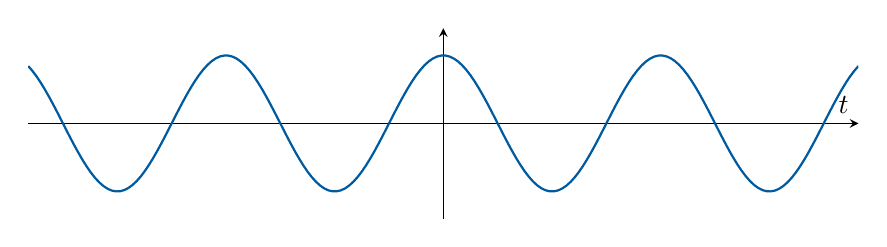
\begin{tikzpicture}
        \begin{axis}[width=\linewidth,height=4cm,axis lines=middle,
            xlabel={$t$},ticks=none,ymin=-1.4,ymax=1.4]
          \addplot[azul,thick,domain=-6:6,samples=200]{cos(deg(2*x))};
        \end{axis}
      \end{tikzpicture}\\
      $f(t)=\cos\omega_0 t$
    \end{column}
    \begin{column}{0.48\textwidth}
      \centering
      \begin{tikzpicture}
        \draw[-{Stealth}] (-2.6,0)--(2.8,0) node[right]{$\omega$};
        \draw[rojo,very thick,-{Stealth}] (1.4,0)--(1.4,1.8);
        \draw[rojo,very thick,-{Stealth}] (-1.4,0)--(-1.4,1.8);
        \node[below] at (1.4,0) {$\omega_0$};
        \node[below] at (-1.4,0) {$-\omega_0$};
      \end{tikzpicture}\\[2mm]
      $F(\omega)$
    \end{column}
  \end{columns}
  \vspace{5mm}
  A tuning fork, a string or an ideal spring oscillates at a single frequency.
  The Fourier transform is the tool that tells us which frequencies a signal contains.
  For the sine and the cosine we expect ``just one'', and we will see that the
  mathematical answer is two Dirac deltas, at $+\omega_0$ and at $-\omega_0$.
\end{frame}

% ------------------------------------------------------------
\begin{frame}{The idea behind the transform}
  To find out whether a signal $f(t)$ contains the frequency $\omega$, we multiply it by an
  oscillation of that frequency and integrate.
  \begin{columns}[c]
    \begin{column}{0.48\textwidth}
      \centering
      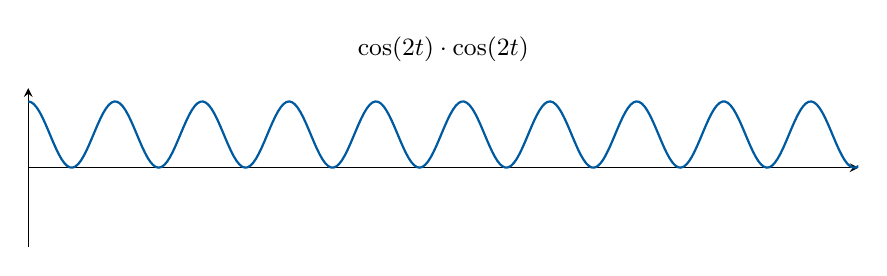
\begin{tikzpicture}
        \begin{axis}[width=\linewidth,height=3.6cm,axis lines=middle,
            ticks=none,ymin=-1.2,ymax=1.2,xmin=0,xmax=15,
            title={\small $\cos(2t)\cdot\cos(2t)$}]
          \addplot[azul,thick,domain=0:15,samples=300]{cos(deg(2*x))*cos(deg(2*x))};
        \end{axis}
      \end{tikzpicture}\\
      {\small Same frequency: the product is always positive and the integral grows.}
    \end{column}
    \begin{column}{0.48\textwidth}
      \centering
      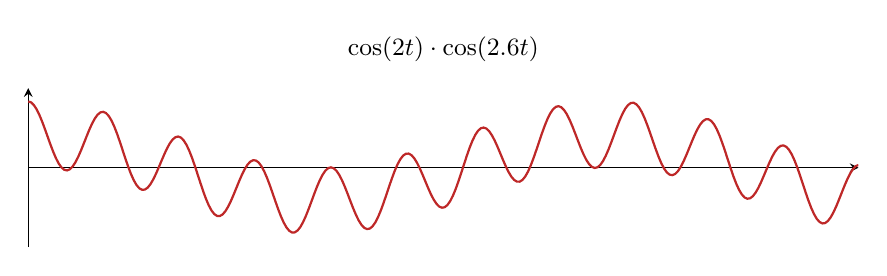
\begin{tikzpicture}
        \begin{axis}[width=\linewidth,height=3.6cm,axis lines=middle,
            ticks=none,ymin=-1.2,ymax=1.2,xmin=0,xmax=15,
            title={\small $\cos(2t)\cdot\cos(2.6t)$}]
          \addplot[rojo,thick,domain=0:15,samples=300]{cos(deg(2*x))*cos(deg(2.6*x))};
        \end{axis}
      \end{tikzpicture}\\
      {\small Different frequencies: the product changes sign and the integral cancels on average.}
    \end{column}
  \end{columns}
  \vspace{3mm}
  So that we don't have to test with sine and cosine separately, we use the complex
  exponential $\e^{-\ii\omega t}=\cos\omega t-\ii\sin\omega t$, which contains both.
\end{frame}

% ------------------------------------------------------------
\begin{frame}{Definition}
  With that idea we define
  \[
    F(\omega)=\int_{-\infty}^{\infty} f(t)\,\e^{-\ii\omega t}\dd t .
  \]
  In general $F(\omega)$ is a complex number: its modulus tells us how much of the
  frequency $\omega$ there is, and its argument tells us with what phase it appears.

  \vspace{3mm}
  The signal is recovered with the inverse transform,
  \[
    f(t)=\frac{1}{2\pi}\int_{-\infty}^{\infty} F(\omega)\,\e^{\ii\omega t}\dd\omega ,
  \]
  which reads as ``$f$ is a sum (integral) of oscillations $\e^{\ii\omega t}$, each one
  with weight $F(\omega)/2\pi$''.

  \vspace{3mm}
  {\small Other books put the factor $2\pi$ somewhere else, or use the frequency $f$ in Hz
  with $\e^{-2\pi\ii ft}$. The constants change, not the form of the results.}
\end{frame}

% ------------------------------------------------------------
\begin{frame}{The cosine as a sum of two phasors}
  \begin{columns}[c]
    \begin{column}{0.55\textwidth}
      From Euler's formula, $\e^{\pm\ii\theta}=\cos\theta\pm\ii\sin\theta$, we get
      \[
        \cos\omega_0 t=\frac{\e^{\ii\omega_0 t}+\e^{-\ii\omega_0 t}}{2},\qquad
        \sin\omega_0 t=\frac{\e^{\ii\omega_0 t}-\e^{-\ii\omega_0 t}}{2\ii}.
      \]
      $\e^{\ii\omega_0 t}$ is a vector of length 1 that rotates counterclockwise with
      angular velocity $\omega_0$, and $\e^{-\ii\omega_0 t}$ rotates clockwise.

      \vspace{2mm}
      When we add them, the imaginary parts cancel and what is left is a real number
      oscillating along the horizontal axis: the cosine. That is why both frequencies,
      $+\omega_0$ and $-\omega_0$, will appear in the spectrum.
    \end{column}
    \begin{column}{0.42\textwidth}
      \centering
      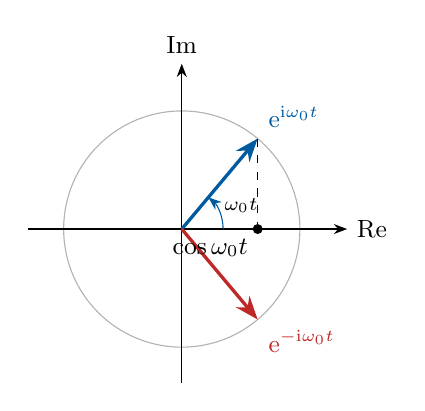
\begin{tikzpicture}[scale=1.5]
        \draw[gray!60] (0,0) circle (1);
        \draw[-{Stealth}] (-1.3,0)--(1.4,0) node[right]{\small Re};
        \draw[-{Stealth}] (0,-1.3)--(0,1.4) node[above]{\small Im};
        \draw[azul,very thick,-{Stealth}] (0,0)--(50:1) node[above right]{\small$\e^{\ii\omega_0 t}$};
        \draw[rojo,very thick,-{Stealth}] (0,0)--(-50:1) node[below right]{\small$\e^{-\ii\omega_0 t}$};
        \draw[dashed] (50:1)--({cos(50)},0);
        \fill (({cos(50)},0) circle (1.2pt);
        \node[below left] at ({cos(50)},0) {\small$\cos\omega_0 t$};
        \draw[azul,-{Stealth}] (0.35,0) arc (0:50:0.35);
        \node at (0.5,0.2) {\scriptsize$\omega_0 t$};
      \end{tikzpicture}
    \end{column}
  \end{columns}
\end{frame}

% ------------------------------------------------------------
\begin{frame}{The problem: the integral does not converge}
  If we try to compute the transform directly:
  \[
    \int_{-\infty}^{\infty}\cos(\omega_0 t)\,\e^{-\ii\omega t}\dd t
    =\frac12\int_{-\infty}^{\infty}\e^{-\ii(\omega-\omega_0)t}\dd t
     +\frac12\int_{-\infty}^{\infty}\e^{-\ii(\omega+\omega_0)t}\dd t
  \]
  Both integrals are of the same type, $\int_{-\infty}^{\infty}\e^{-\ii\Omega t}\dd t$:
  \begin{itemize}
    \item if $\Omega\neq0$, the integrand keeps rotating and does not decay, so the integral
          oscillates and has no limit;
    \item if $\Omega=0$, the integrand equals 1 everywhere and the integral is infinite.
  \end{itemize}

  \vspace{2mm}
  The root of the problem is that the cosine lasts forever and does not decay:
  $\int|\cos\omega_0 t|\dd t=\infty$. The usual transform is only guaranteed to exist for
  integrable functions.

  \vspace{2mm}
  To get around this, we observe the signal for a finite time, compute the transform
  (which does exist), and then let that time grow.
\end{frame}

% ------------------------------------------------------------
\begin{frame}{Finite window: the calculation}
  We integrate only between $-T$ and $T$:
  \begin{align*}
    \int_{-T}^{T}\e^{-\ii\Omega t}\dd t
    &=\left[\frac{\e^{-\ii\Omega t}}{-\ii\Omega}\right]_{-T}^{T}
     =\frac{\e^{-\ii\Omega T}-\e^{\ii\Omega T}}{-\ii\Omega}\\[1mm]
    &=\frac{-2\ii\sin(\Omega T)}{-\ii\Omega}
     =\frac{2\sin(\Omega T)}{\Omega}.
  \end{align*}
  In the second line we used $\e^{\ii a}-\e^{-\ii a}=2\ii\sin a$.

  \vspace{3mm}
  We call $D_T(\Omega)=\dfrac{2\sin(\Omega T)}{\Omega}$. The result is now an ordinary
  function; what remains is to see what happens to it as $T\to\infty$.
\end{frame}

% ------------------------------------------------------------
\begin{frame}{Finite window: what happens to $D_T$}
  \begin{columns}[c]
    \begin{column}{0.5\textwidth}
      \begin{itemize}
        \item \textbf{Height.} Near $\Omega=0$, $\sin(\Omega T)\approx\Omega T$, so
              $D_T(0)=2T$. It grows without bound.
        \medskip
        \item \textbf{Width.} The first zero is where $\Omega T=\pi$, that is, $\Omega=\pi/T$.
              The peak gets narrower.
        \medskip
        \item \textbf{Area.} With $u=\Omega T$,
              \[
                \int_{-\infty}^{\infty}\frac{2\sin\Omega T}{\Omega}\dd\Omega
                =2\int_{-\infty}^{\infty}\frac{\sin u}{u}\dd u=2\pi,
              \]
              which does not depend on $T$.
      \end{itemize}
    \end{column}
    \begin{column}{0.48\textwidth}
      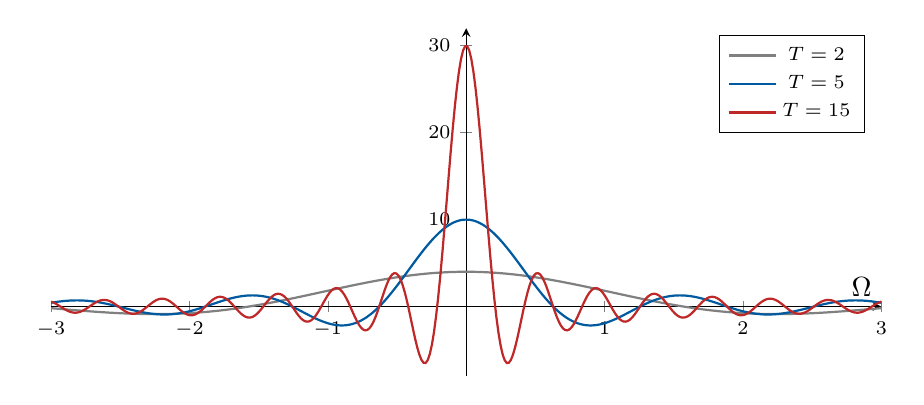
\begin{tikzpicture}
        \begin{axis}[width=\linewidth,height=6cm,axis lines=middle,
            xlabel={$\Omega$},ymin=-8,ymax=32,xmin=-3,xmax=3,
            legend style={font=\scriptsize,at={(0.98,0.98)},anchor=north east},
            tick label style={font=\scriptsize}]
          \addplot[gray,thick,domain=-3:3,samples=400]{2*sin(deg(x*2))/x};
          \addplot[azul,thick,domain=-3:3,samples=400]{2*sin(deg(x*5))/x};
          \addplot[rojo,thick,domain=-3:3,samples=400]{2*sin(deg(x*15))/x};
          \legend{$T=2$,$T=5$,$T=15$}
        \end{axis}
      \end{tikzpicture}
    \end{column}
  \end{columns}
  \vspace{2mm}
  A peak that gets taller and narrower, but with a fixed area $2\pi$: that is exactly what
  defines a Dirac delta.
\end{frame}

% ------------------------------------------------------------
\begin{frame}{The Dirac delta}
  $\delta(\Omega)$ is not a function in the usual sense. It is defined by what it does inside
  an integral:
  \[
    \int_{-\infty}^{\infty}\delta(\Omega)\,\varphi(\Omega)\dd\Omega=\varphi(0)
    \qquad\text{for every smooth function }\varphi .
  \]
  Properties we will use:
  \[
    \int_{-\infty}^{\infty}\delta(\Omega)\dd\Omega=1,
    \qquad
    g(\Omega)\,\delta(\Omega-a)=g(a)\,\delta(\Omega-a).
  \]

  \vspace{2mm}
  Back to the window: as $T\to\infty$, $D_T$ concentrates at $\Omega=0$ with area
  $2\pi$, so that
  \[
    \int_{-\infty}^{\infty}D_T(\Omega)\,\varphi(\Omega)\dd\Omega\;\longrightarrow\;2\pi\,\varphi(0)
    \qquad\Longrightarrow\qquad
    \boxed{\int_{-\infty}^{\infty}\e^{-\ii\Omega t}\dd t=2\pi\,\delta(\Omega)}
  \]
\end{frame}

% ------------------------------------------------------------
\begin{frame}{Transform of the cosine}
  We start from
  \[
    \cos\omega_0 t=\tfrac12\,\e^{\ii\omega_0 t}+\tfrac12\,\e^{-\ii\omega_0 t}.
  \]
  The transform of each exponential follows from the previous result with $\Omega=\omega\mp\omega_0$:
  \[
    \F\{\e^{\ii\omega_0 t}\}=\int_{-\infty}^{\infty}\e^{-\ii(\omega-\omega_0)t}\dd t=2\pi\,\delta(\omega-\omega_0),
    \qquad
    \F\{\e^{-\ii\omega_0 t}\}=2\pi\,\delta(\omega+\omega_0).
  \]
  Since the transform is linear,
  \[
    \boxed{\F\{\cos\omega_0 t\}=\pi\left[\delta(\omega-\omega_0)+\delta(\omega+\omega_0)\right]}
  \]
  To check it, we apply the inverse transform and use the property of the delta:
  \[
    \frac{1}{2\pi}\int_{-\infty}^{\infty}\pi\left[\delta(\omega-\omega_0)+\delta(\omega+\omega_0)\right]\e^{\ii\omega t}\dd\omega
    =\frac{\e^{\ii\omega_0 t}+\e^{-\ii\omega_0 t}}{2}=\cos\omega_0 t .
  \]
\end{frame}

% ------------------------------------------------------------
\begin{frame}{Transform of the sine}
  The procedure is the same:
  \[
    \sin\omega_0 t=\frac{1}{2\ii}\,\e^{\ii\omega_0 t}-\frac{1}{2\ii}\,\e^{-\ii\omega_0 t}
    \quad\Longrightarrow\quad
    \F\{\sin\omega_0 t\}=\frac{2\pi}{2\ii}\left[\delta(\omega-\omega_0)-\delta(\omega+\omega_0)\right].
  \]
  Multiplying numerator and denominator by $\ii$ gives $\dfrac{1}{\ii}=-\ii$, so
  \[
    \boxed{\F\{\sin\omega_0 t\}=\ii\pi\left[\delta(\omega+\omega_0)-\delta(\omega-\omega_0)\right]}
  \]
  Check:
  \[
    \frac{1}{2\pi}\,(\ii\pi)\left(\e^{-\ii\omega_0 t}-\e^{\ii\omega_0 t}\right)
    =\frac{\ii}{2}\left(-2\ii\sin\omega_0 t\right)=\sin\omega_0 t .
  \]
  Unlike the cosine, the result is purely imaginary.
\end{frame}

% ------------------------------------------------------------
\begin{frame}{Comparing the two spectra}
  \begin{columns}[T]
    \begin{column}{0.48\textwidth}
      \centering
      Cosine\\[1mm]
      \begin{tikzpicture}[scale=0.85]
        \draw[-{Stealth}] (-3,0)--(3.2,0) node[right]{$\omega$};
        \draw[-{Stealth}] (0,-1.7)--(0,2) node[above]{$\operatorname{Re}F$};
        \draw[azul,ultra thick,-{Stealth}] (1.5,0)--(1.5,1.4) node[above]{$\pi$};
        \draw[azul,ultra thick,-{Stealth}] (-1.5,0)--(-1.5,1.4) node[above]{$\pi$};
        \node[below] at (1.5,0) {$\omega_0$};
        \node[below] at (-1.5,0) {$-\omega_0$};
      \end{tikzpicture}
    \end{column}
    \begin{column}{0.48\textwidth}
      \centering
      Sine\\[1mm]
      \begin{tikzpicture}[scale=0.85]
        \draw[-{Stealth}] (-3,0)--(3.2,0) node[right]{$\omega$};
        \draw[-{Stealth}] (0,-1.7)--(0,2) node[above]{$\operatorname{Im}F$};
        \draw[rojo,ultra thick,-{Stealth}] (-1.5,0)--(-1.5,1.4) node[above]{$\pi$};
        \draw[rojo,ultra thick,-{Stealth}] (1.5,0)--(1.5,-1.4) node[below]{$-\pi$};
        \node[below] at (-1.5,0) {$-\omega_0$};
        \node[above] at (1.5,0) {$\omega_0$};
      \end{tikzpicture}
    \end{column}
  \end{columns}
  \vspace{4mm}
  \begin{itemize}
    \item Same frequencies and same $|F(\omega)|$; only the phase changes.
    \item Even cosine $\Rightarrow$ real and even transform. Odd sine $\Rightarrow$
          imaginary and odd transform.
    \item The height of each arrow is the weight (area) of the delta.
  \end{itemize}
\end{frame}

% ------------------------------------------------------------
\begin{frame}{Interpretation}
  \textbf{Negative frequencies.} They are not a different physical thing: they appear because
  we write a real signal with complex exponentials, and both directions of rotation are needed
  for the sum to be real. Every real signal satisfies $F(-\omega)=\overline{F(\omega)}$,
  so the negative part carries no new information.

  \vspace{3mm}
  \textbf{The phase.} The sine is a delayed cosine: $\sin\omega_0 t=\cos\big(\omega_0(t-t_0)\big)$
  with $t_0=\pi/(2\omega_0)$. A delay $t_0$ multiplies the transform by
  $\e^{-\ii\omega t_0}$, which at $\omega=\pm\omega_0$ equals $\e^{\mp\ii\pi/2}=\mp\ii$.
  That explains the factors of $\ii$ in the sine: the frequencies do not change, only the phase.

  \vspace{3mm}
  \textbf{Why deltas?} An oscillation that never ends has infinite total energy,
  but finite average power, $\langle A^2\cos^2\omega_0 t\rangle=A^2/2$. All that power
  sits at a single frequency, and a finite amount concentrated at one point is exactly
  a delta.
\end{frame}

% ============================================================
\section{Application}

\begin{frame}{Application: the driven oscillator}
  \begin{columns}[c]
    \begin{column}{0.6\textwidth}
      A block attached to a spring, with friction, is pushed by a periodic force:
      \[
        m\,\ddot x+b\,\dot x+k\,x=F_0\cos(\Omega t).
      \]
      With what amplitude and what phase does the block oscillate?

      \vspace{3mm}
      Values: $m=\SI{0.5}{kg}$, $k=\SI{20}{N/m}$, $b=\SI{0.5}{kg/s}$, $F_0=\SI{1}{N}$.
    \end{column}
    \begin{column}{0.37\textwidth}
      \centering
      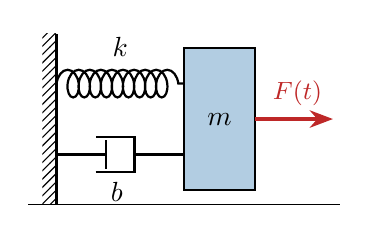
\begin{tikzpicture}[scale=0.9]
        \fill[pattern=north east lines] (-0.2,-0.2) rectangle (0,2.2);
        \draw[thick] (0,-0.2)--(0,2.2);
        \draw[thick,decorate,decoration={coil,aspect=0.6,segment length=4pt,amplitude=5pt}] (0,1.5)--(1.8,1.5);
        \node[above] at (0.9,1.75) {$k$};
        \draw[thick] (0,0.5)--(0.7,0.5);
        \draw[thick] (0.7,0.3)--(0.7,0.7);
        \draw[thick] (0.55,0.25)--(1.1,0.25)--(1.1,0.75)--(0.55,0.75);
        \draw[thick] (1.1,0.5)--(1.8,0.5);
        \node[below] at (0.85,0.25) {$b$};
        \draw[thick,fill=azul!30] (1.8,0) rectangle (2.8,2);
        \node at (2.3,1) {$m$};
        \draw[rojo,very thick,-{Stealth}] (2.8,1)--(3.9,1);
        \node[rojo,above] at (3.4,1.05) {\small$F(t)$};
        \draw (-0.4,-0.2)--(4,-0.2);
      \end{tikzpicture}
    \end{column}
  \end{columns}
\end{frame}

% ------------------------------------------------------------
\begin{frame}{Transforming the equation}
  Differentiating $\e^{\ii\omega t}$ is the same as multiplying it by $\ii\omega$, so
  \[
    \F\{\dot x\}=\ii\omega X(\omega),\qquad \F\{\ddot x\}=-\omega^2X(\omega).
  \]
  We apply $\F$ to the equation and use the transform of the cosine on the right-hand side:
  \[
    \left(k-m\omega^2+\ii b\omega\right)X(\omega)
    =\pi F_0\left[\delta(\omega-\Omega)+\delta(\omega+\Omega)\right].
  \]
  With $H(\omega)=k-m\omega^2+\ii b\omega$:
  \[
    X(\omega)=\frac{\pi F_0}{H(\omega)}\left[\delta(\omega-\Omega)+\delta(\omega+\Omega)\right].
  \]
  The differential equation has become an algebraic one.
\end{frame}

% ------------------------------------------------------------
\begin{frame}{Back to the time domain}
  In the inverse transform, the deltas do all the work:
  \[
    x(t)=\frac{1}{2\pi}\int_{-\infty}^{\infty}X(\omega)\,\e^{\ii\omega t}\dd\omega
    =\frac{F_0}{2}\left[\frac{\e^{\ii\Omega t}}{H(\Omega)}+\frac{\e^{-\ii\Omega t}}{H(-\Omega)}\right]
    =\operatorname{Re}\!\left[\frac{F_0\,\e^{\ii\Omega t}}{H(\Omega)}\right],
  \]
  because the two terms are complex conjugates. Writing $H(\Omega)=|H|\e^{\ii\varphi}$:
  \[
    \boxed{x(t)=A\cos(\Omega t-\varphi)},\qquad
    A=\frac{F_0}{\sqrt{(k-m\Omega^2)^2+(b\Omega)^2}},\qquad
    \tan\varphi=\frac{b\Omega}{k-m\Omega^2}.
  \]
  \vspace{1mm}
  The block oscillates at the frequency of the force. At resonance, $\Omega=\omega_0=\sqrt{k/m}$,
  the amplitude is largest and the phase lag is $90^\circ$. With a force $F_0\sin(\Omega t)$ we
  use the transform of the sine and get $A\sin(\Omega t-\varphi)$.
\end{frame}

% ------------------------------------------------------------
\begin{frame}[fragile]{Checking with Python}
  \begin{columns}[T]
    \begin{column}{0.63\textwidth}
      \vspace*{-4mm}
      \lstinputlisting[lastline=26]{forced_oscillator.py}
    \end{column}
    \begin{column}{0.34\textwidth}
      \small
      Fourier assumes the force has been acting forever. With Python we solve the full
      equation starting from rest, $x(0)=\dot x(0)=0$, and compare.

      \vspace{3mm}
      Program output at resonance:
      \begin{center}
        \begin{tabular}{lr}
          \toprule
          $A$ Fourier & \SI{0.3162}{m}\\
          $A$ numerical & \SI{0.3162}{m}\\
          $\varphi$ & $90.0^\circ$\\
          \bottomrule
        \end{tabular}
      \end{center}
    \end{column}
  \end{columns}
\end{frame}

% ------------------------------------------------------------
\begin{frame}{Result}
  \centering
  \includegraphics[width=0.85\linewidth]{forced_oscillator.png}

  \vspace{2mm}
  \raggedright
  At first the numerical solution grows from zero: this is the transient, which depends on
  how the system starts and dies out because of friction. After about \SI{10}{s} the two
  curves coincide, and the Fourier transform gives the steady motion exactly.
\end{frame}

% ------------------------------------------------------------
\begin{frame}{Conclusions}
  \begin{itemize}
    \item The Fourier integral of the sine and the cosine does not converge in the usual sense;
          observing the signal for a finite time $T$ and letting $T\to\infty$ gives two
          deltas at $\pm\omega_0$.
    \medskip
    \item The sine and the cosine have the same modulus. The cosine gives a real spectrum and
          the sine an imaginary one: only the phase changes.
    \medskip
    \item In the driven oscillator, the transform of the cosine turns the differential equation
          into an algebraic one, and the deltas solve the inverse transform.
          Python confirms the result once the transient has passed.
  \end{itemize}
\end{frame}

% ------------------------------------------------------------
\begin{frame}{References}
  \small
  \begin{itemize}
    \item R.~N.~Bracewell, \emph{The Fourier Transform and Its Applications},
          3rd ed., McGraw-Hill, 2000.
    \item G.~B.~Arfken, H.~J.~Weber and F.~E.~Harris, \emph{Mathematical Methods for Physicists},
          7th ed., Academic Press, 2013. Ch.~20.
    \item J.~R.~Taylor, \emph{Classical Mechanics}, University Science Books, 2005. Ch.~5
          (driven oscillations and resonance).
    \item A.~P.~French, \emph{Vibrations and Waves}, W.~W.~Norton, 1971.
    \item SciPy documentation, \texttt{scipy.integrate.solve\_ivp}:
          \texttt{docs.scipy.org}.
  \end{itemize}
\end{frame}

\begin{frame}
  \centering
  \vfill
  {\Large Thank you}
  \vfill
\end{frame}

\end{document}
